%%**************************************************************
%% Vorlage fuer Bachelorarbeiten (o.ä.) der DHBW
%%
%% Autor: Tobias Dreher, Yves Fischer
%% Datum: 06.07.2011
%%**************************************************************

\newcommand{\pdftitel}{Programmentwurf Teil 1}
\newcommand{\autor}{Christian Burkard \& Florian Kanngiesser}
\newcommand{\arbeit}{Aufgabenteil E\_002}

%
% Nahezu alle Einstellungen koennen hier getaetigt werden
%

\documentclass[%
	pdftex,
	oneside,		% Einseitiger Druck.
	12pt,			% Schriftgroesse
	parskip=half,	% Halbe Zeile Abstand zwischen Absätzen.
	headsepline,	% Linie nach Kopfzeile.
	footsepline,	% Linie vor Fusszeile.
	abstracton,	    % Abstract Überschriften
	ngerman,		% Translator
]{scrreprt}

%Seitengroesse
\usepackage{fullpage}

%Zeilenumbruch und mehr
\usepackage[activate]{microtype}

% Zeichencodierung
\usepackage[utf8]{inputenc}
\usepackage[T1]{fontenc}

% Zeilenabstand
\usepackage[onehalfspacing]{setspace}

% Index-Erstellung
\usepackage{makeidx}

% Lokalisierung (neue deutsche Rechtschreibung)
%\usepackage[english]{babel}
\usepackage[ngerman]{babel} 

% Anführungszeichen 
\usepackage[babel,german=quotes]{csquotes}
%\usepackage[style=swiss]{csquotes}


% Spezielle Tabellenform fuer Deckblatt
\usepackage{longtable}
\setlength{\tabcolsep}{10pt} %Abstand zwischen Spalten
\renewcommand{\arraystretch}{1.5} %Zeilenabstand

% Grafiken
\usepackage{graphicx}

% Mathematische Textsaetze
%\usepackage{amsmath}
%\usepackage{amssymb}

% Pakete um Textteile drehen zu können, oder eine Seite Querformat anzeigen kann.
%\usepackage{rotating}
%\usepackage{lscape}

% Farben
\usepackage{color}
\definecolor{LinkColor}{rgb}{0,0,0.2}
\definecolor{ListingBackground}{rgb}{0.92,0.92,0.92}

% PDF Einstellungen
\usepackage[%
	pdftitle={\pdftitel},
	pdfauthor={\autor},
	pdfsubject={\arbeit},
	pdfcreator={pdflatex, LaTeX with KOMA-Script},
	pdfpagemode=UseOutlines, % Beim Oeffnen Inhaltsverzeichnis anzeigen
	pdfdisplaydoctitle=true, % Dokumenttitel statt Dateiname anzeigen.
	pdflang=en % Sprache des Dokuments.
]{hyperref}

% (Farb-)einstellungen für die Links im PDF
\hypersetup{%
	colorlinks=false, % Aktivieren von farbigen Links im Dokument
	linkcolor=LinkColor, % Farbe festlegen
	citecolor=LinkColor,
	filecolor=LinkColor,
	menucolor=LinkColor,
	urlcolor=LinkColor,
	bookmarksnumbered=true % Überschriftsnummerierung im PDF Inhalt anzeigen.
}

% Verschiedene Schriftarten
%\usepackage{goudysans}
%\usepackage{lmodern}
%\usepackage{libertine}
\usepackage{palatino} 

% Hurenkinder und Schusterjungen verhindern
% http://projekte.dante.de/DanteFAQ/Silbentrennung
\clubpenalty=10000
\widowpenalty=10000
\displaywidowpenalty=10000

% Quellcode
\usepackage{listings}
\lstloadlanguages{Java}
\lstset{%
	language=Java,		 	 % Sprache des Quellcodes
	numbers=left,           % Zelennummern links
	stepnumber=1,            % Jede Zeile nummerieren.
	numbersep=5pt,           % 5pt Abstand zum Quellcode
	numberstyle=\tiny,       % Zeichengrösse 'tiny' für die Nummern.
	breaklines=true,         % Zeilen umbrechen wenn notwendig.
	breakautoindent=true,    % Nach dem Zeilenumbruch Zeile einrücken.
	postbreak=\space,        % Bei Leerzeichen umbrechen.
	tabsize=2,               % Tabulatorgrösse 2
	basicstyle=\ttfamily\footnotesize, % Nichtproportionale Schrift, klein für den Quellcode
	showspaces=false,        % Leerzeichen nicht anzeigen.
	showstringspaces=false,  % Leerzeichen auch in Strings ('') nicht anzeigen.
	extendedchars=true,      % Alle Zeichen vom Latin1 Zeichensatz anzeigen.
	captionpos=b,            % sets the caption-position to bottom
	backgroundcolor=\color{ListingBackground} % Hintergrundfarbe des Quellcodes setzen.
}
% Deutsche Überschriften im Appendix
\addto{\captionsngerman}{
  \renewcommand{\contentsname}{\sffamily Inhaltsverzeichnis}
  \renewcommand{\listfigurename}{\sffamily Abbildungsverzeichnis}
  \renewcommand{\lstlistingname}{\sffamily Quellcodeverzeichnis}
  \renewcommand{\lstlistlistingname}{\sffamily Quellcodeverzeichnis}
}


% Glossar
\usepackage[
	nonumberlist, %keine Seitenzahlen anzeigen
	acronym,      %ein Abkürzungsverzeichnis erstellen
	section,      %im Inhaltsverzeichnis auf section-Ebene erscheinen
	toc,          %Einträge im Inhaltsverzeichnis
]{glossaries}

% Fussnoten
\usepackage[perpage, hang, multiple, stable]{footmisc}

% Seitenränder
\usepackage{anysize}
\marginsize{30mm}{25mm}{25mm}{25mm}

% Titel, Autor und Datum
\title{\titel}
\author{\autor}
\date{\datum}
 

% Ab jetzt können auch Umlaute verwendet werden
\newcommand{\titel}{Entwicklung eines Online Kochbuchs mithilfe von Java Server Pages und Hibernate}
\newcommand{\martrikelnr}{4206853 \& 7353550}
\newcommand{\kurs}{TITAIA2010}
\newcommand{\datumAbgabe}{Juni 2012}
\newcommand{\abgabeort}{Stuttgart}
\newcommand{\studiengang}{Studiengang Angewandte Informatik}
\newcommand{\dhbw}{Stuttgart}
\newcommand{\betreuer}{Prof. Dr. Dirk Reichardt}
%\newcommand{\zeitraum}{}

\makeglossaries
%
% vorher in Konsole folgendes aufrufen: 
%	makeglossaries makeglossaries dokumentation.acn && makeglossaries dokumentation.glo
%

% 
% Abkürzungen --> referenz, name, beschreibung
% Aufruf mit \gls{...} oder Kurzform mit \acrshort{...}
%
\newacronym{jsp}{JSP}{Java Server Pages}
\newacronym{mvc}{MVC}{Model-View-Controller}
\newacronym{xml}{XML}{Extensible Markup Language}
\newacronym{html}{HTML}{Hypertext Markup Language}




%
% Glossareintraege --> referenz, name, beschreibung
% Aufruf mit \gls{...}
%

\newglossaryentry{mysql}{name={MySQL},description={Eine sehr weit verbreitete, relationale Open-Source-Datenbank}}
\newglossaryentry{hibernate}{name={Hibernate},description={Ein Open-Source Framework, mit Object-Relational-Mapping für Java Anwendungen}}



\begin{document}

	% Deckblatt
	\begin{spacing}{1}
		\begin{titlepage}
	\begin{longtable}{p{.55\textwidth} p{.85\textwidth}}
	  {
\includegraphics[height=2.6cm]{images/logo.png}} & 
	  {
\includegraphics[height=2.6cm]{images/dhbw.png}}
	\end{longtable}
	\enlargethispage{20mm}
	\begin{center}
	  \vspace*{12mm}	{\LARGE\bf \titel }\\
	  \vspace*{12mm}	{\large\bf \arbeit}\\
	  \vspace*{12mm}	Dokumentation für Wissensbasierte Systeme im \studiengang\\
	  \vspace*{3mm} 	an der Dualen Hochschule Baden-Württemberg \dhbw\\
	  \vspace*{12mm}	von\\
	  \vspace*{3mm} 	{\large\bf \autor}\\
	  \vspace*{12mm}	\datumAbgabe\\
	\end{center}
	\vfill
	\begin{spacing}{1.2}
	\begin{tabbing}
		mmmmmmmmmmmmmmmmmmmmmmmmmm     \= \kill
		%\textbf{Bearbeitungszeitraum}  \>  \zeitraum\\
		\textbf{Matrikelnummer, Kurs}  \>  \martrikelnr, \kurs\\
		\textbf{Betreuer}              \>  \betreuer\\
	\end{tabbing}
	\end{spacing}
\end{titlepage}

	\end{spacing}
	\newpage
	
	\renewcommand{\thepage}{\Roman{page}}
	\setcounter{page}{1}	

	% Erklärung
	%\thispagestyle{empty}

\section*{Erklärung}
% Seite 8
% http://studium.ba-bw.de/fileadmin/media/allgemein/bestimmungen/btechnik/richtlinien/Richtlinien_Praxismodule_Studien_und_Bachelorarbeiten_2011.pdf
\vspace*{2em}

gemäß § 5 (2) der „Studien- und Prüfungsordnung DHBW Technik“ vom 18. Mai 2009.

Ich habe die vorliegende Arbeit selbstständig verfasst und keine anderen als die angegebenen
Quellen und Hilfsmittel verwendet.
\vspace{3em}

\abgabeort, \datumAbgabe
\vspace{4em}

\autor


	%\newpage

	% Abstract
	%\thispagestyle{empty}

\renewcommand{\abstractname}{Zusammenfassung}
\begin{abstract}
Ein Abstract ist eine prägnante Inhaltsangabe, ein Abriss ohne
Interpretation und Wertung einer wissenschaftlichen Arbeit. In DIN
1426 wird das (oder auch der) Abstract als Kurzreferat zur
Inhaltsangabe beschrieben.

\begin{description}
\item[Objektivität] soll sich jeder persönlichen Wertung enthalten
\item[Kürze] soll so kurz wie möglich sein
\item[Genauigkeit] soll genau die Inhalte und die Meinung der Originalarbeit wiedergeben
\end{description}

Üblicherweise müssen wissenschaftliche Artikel einen Abstract
enthalten, typischerweise von 100-150 Wörtern, ohne Bilder und
Literaturzitate und in einem Absatz.

Quelle \url{http://de.wikipedia.org/wiki/Abstract} Abgerufen 07.07.2011
\end{abstract}


\renewcommand{\abstractname}{Summary}
\begin{abstract}
An abstract is a brief summary of a research article, thesis, review,
conference proceeding or any in-depth analysis of a particular subject
or discipline, and is often used to help the reader quickly ascertain
the paper's purpose. When used, an abstract always appears at the
beginning of a manuscript, acting as the point-of-entry for any given
scientific paper or patent application. Abstracting and indexing
services for various academic disciplines are aimed at compiling a
body of literature for that particular subject.

The terms précis or synopsis are used in some publications to refer to
the same thing that other publications might call an "abstract". In
management reports, an executive summary usually contains more
information (and often more sensitive information) than the abstract
does.

Quelle: \url{http://en.wikipedia.org/wiki/Abstract_(summary)}

\end{abstract}

	%\newpage

	% Inhaltsverzeichnis
	\begin{spacing}{1.1}
		\setcounter{tocdepth}{2}
		\tableofcontents
	\end{spacing}
	\newpage

	\renewcommand{\thepage}{\arabic{page}}
	\setcounter{page}{1}
	
	% Inhalt
	\chapter{Einführung}
Anders als im Readme beschrieben haben wir uns für einen
einzigen File als Input entschieden. Der Gründe dafür waren
das im ersten Beispiel nur eine einzige Datei vorlag und wir
deshalb unseren ursprünglichen Entwurf darauf ausgelegt hatten.
Außerdem spielt es auch keine Rolle ob man ein oder zwei
Dateien verwendet.\\
\section{Input File Format}
  Das Input-File ist in 2 Sektionen unterteilt, welche mittels
  Semikolon voneinander getrennt sind. Die einzelnen Attribute
  werden mittels Komma separiert.\\
  Aus diesem Format sind wir nun in der Lage Primitive und
  Relationen zu generieren.
  Zuerst werden die Primitive ausgelesen und in eine geeignete
  Datenstruktur gespeichert, anschließend die Relationen.
	\chapter{Datenbankschnittstelle: \gls{hibernate}}
Dieses Kapitel behandelt die Datenbankanbindung der Kochbuchanwendung.
\section{Object-Relational Mapping (ORM)}
\gls{hibernate} bietet die Möglichkeit relationale Datenbankstrukturen auf Java Objekte zu mappen. Betrachtet man das ER-Model der Datenbank (s. Abb. \ref{hib_erm}) und das UML Diagramm der Modellschicht (s. Abb. \ref{hib_uml}), fällt einem sofort die strukturelle Ähnlichkeit auf. \gls{hibernate} bietet die Möglichkeit mithilfe eines Mappings durch \acrshort{xml} Files die Modellschicht direkt auf das relationale Schema der Datenbank abzubilden.
\begin{figure}[htbp]
    \centering
    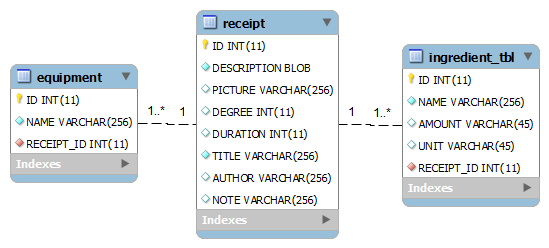
\includegraphics[scale=0.7]{images/relational-model.png}
    \caption{ER-Model der Kochbuch Datenbank}
    \label{hib_erm}
\end{figure}
\begin{figure}[htbp]
    \centering
    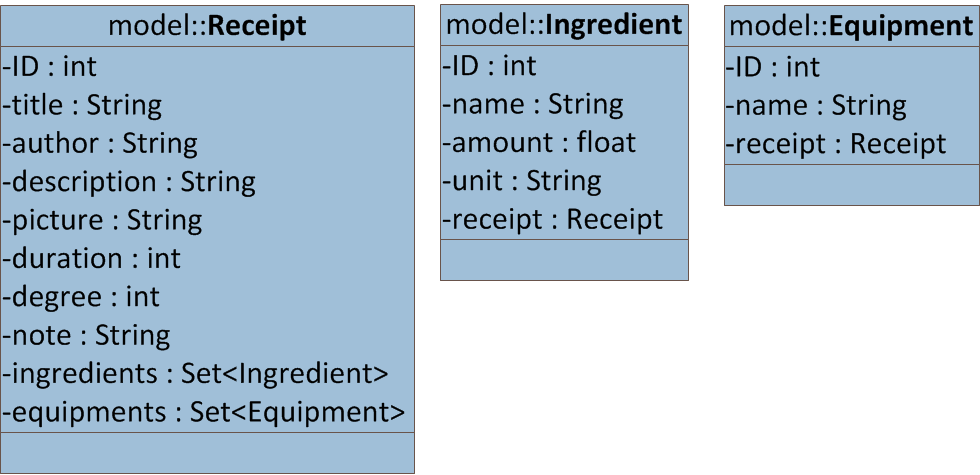
\includegraphics[scale=3.5]{images/model-uml.png}
    \caption{UML der Klassen der Modellschicht}
    \label{hib_uml}
\end{figure}

\section{Klassen - Tabellen Mapping}
Wie in Abbildung \ref{hib_erm} und \ref{hib_uml} zu sehen ist werden drei Klassen auf drei Tabellen abgebildet. Jeweils eine Klasse wird auf eine Tabelle abgebildet. ($Namentlich: Receipt \rightarrow receipt, Ingredient \rightarrow ingredient\_tbl \ und \  Equipment \rightarrow equipment$)
Das Mapping findet statt, indem für jede Klasse, die auf eine Tabelle abgebildet werden soll, eine \acrshort{xml} Konfigurationsdatei im selben package wie die Klasse angelegt wird, die dieses Mapping definiert. Heißt die Klasse \textit{"Foo.java"} ist der Name der Konfigurationsdatei \textit{"Foo.hbm.xml"}.
Sie sagt der Klasse auf welche Tabelle sie abgebildet wird. In diesem Mapping können dann Attribute und Relationen für diese Tabelle/Klasse definiert werden.

\section{Mapping einfacher Attribute}
Ein einfaches Attribut wird über das proberty Tag auf eine Tabellenspalte gemappt. Ein solches Beispielmapping eines Attributs sieht man in Quellcode \ref{hib_prop}. Das Attribut \textit{"name"} benennt das Attribut der Klasse. \textit{"column"} nennt die Spalte der Tabelle, auf die das Attribut, das durch \textit{"name"} definiert wird, gemappt wird. \textit{"type"} ist der Datentyp in dem das Attribut aus der Klasse gelesen und in der Datenbank gespeichert wird. Der Datentyp ist weder der der Javaklasse noch der Datentyp der Datenbanktabellenspalte. Es ist ein \gls{hibernate} mapping Typ.
Im Beispiel Quellcode \ref{hib_prop} ist außerdem, ein optionales Attribut \textit{"not-null"} zu sehen. Die vorherigen Attribute waren alle Pflichteingaben, auf die weitere optionale Attribute folgen können. \textit{not-null="true"} erlaubt es nur Werte ungleich null zu der Spalte hinzuzufügen.
\begin{lstlisting}[caption={Mapping eines Attributes},label=hib_prop]
    <property name="title" column="TITLE" type="string" not-null="true" />
\end{lstlisting}

\section{Mapping von Relationen}
In \gls{hibernate} gibt es zwei Möglichkeiten des Mappings für 1:n Beziehungen. Man kann das Mapping aus zwei Perspektiven sehen: one-to-many oder eine many-to-one Relation. In unserem Kochbuch sind die Rezepte 1:n mit den Zutaten verbunden. Es ist eine one-to-many Beziehung. Genauso könnte man sagen sind die Zutaten many-to-one mit den Rezepten verbunden.
So kann man die Beziehung wie in Beispiel Quellcode \ref{hib_otm} als one-to-many Beziehung von Rezepten zu Zutaten beschreiben. Die one-to-many Beziehung wird in der Klasse mithilfe eines HashSets dargestellt. In Hibernate werden Sets mit dem \textit{set} Tag dargestellt. Dieses HashSet wird hier mit dem \textit{"name"} Attribut angesprochen. \textit{"cascade"} und \textit{"lazy"} sind optionale Attribute und beschreiben das Verhalten bei Updates/Löschen (hier: Zutaten werden auch aktualisiert, wenn Rezepte aktualisiert wurden) oder versetzen Transaktionen mit einer Priorität (hier: nur Indizes des Sets werden geladen. Das Objekt selber wird erst bei Bedarf aus der Datenbank geladen. Für große Anwendungen bietet diese Option Performance-Vorteile).
Der Tag \textit{key} mit seinem Attribut \textit{"column"} beschreibt die Spalte in der Tabelle, in der die Relation als Fremdschlüssel gespeichert wird. Das \textit{one-to-many} Tag gibt mit seinem \textit{"class"} Attribut die Klasse in der sie referenziert wird an. Dadurch ist auch die Hibernate Konfigurationsdatei und darin die Tabelle in der Datenbank zu dieser Klasse bekannt.
\begin{lstlisting}[caption={One-To-Many Beziehung von Rezepten zu Zutaten},label=hib_otm]
    <set name="ingredients" cascade="all" lazy="true">
		<key column="RECEIPT_ID" />
		<one-to-many class="model.Ingredient" />
	</set>
\end{lstlisting}
Die andere Richtung beschreibt das Beispiel Quellcode \ref{hib_mto}. Das \textit{"name"} Attribut des \textit{many-to-one} Tags gibt den Namen des Attributs in der Klasse an, die den Fremdschlüssel als Objektreferenz speichert. Das \textit{"class"} Attribut gibt die Klasse auf die die Referenz zeigt an und entspricht dem Datentyp des Java Attributs. \textit{"column"} gibt die Spalte in der Datenbanktabelle an, in der die Referenz über einen Fremdschlüssel abgebildet wird. Nun kommt abschließend noch ein optionales Attribut \textit{"cascade"} und verhält sich wie in Beispiel Quellcode \ref{hib_otm} beschrieben: Bei Updates oder Löschen des referenzierten Tabelle (Rezept) kaskadiert die Aktion. Die Zutaten werden ebenfalls aktualisiert/gelöscht.
\begin{lstlisting}[caption={Many-To-One Beziehung von Zutaten zu Rezepten},label=hib_mto]
    <many-to-one name="receipt" class="model.Receipt" column="RECEIPT_ID" cascade="all" />
\end{lstlisting}

\subsection*{Die Unterschiede der Relationen}
1:1 Relationen verbinden eine Zeile einer Tabelle mit einer Zeile einer anderen Tabelle.
Sobald eine Zeile einer Tabelle mit mehreren Zeilen einer anderen Tabelle verbindet ist es eine 1:n Relation. Bei n:m Relationen werden mehrere Zeilen der einen Tabelle mit mehreren Zeilen einer anderen Tabelle verbunden. Da diese Information jedoch nicht mehr in einer Spalte sinnvoll gespeichert werden kann, benötigt man eine extra Tabelle um diese Verbindungsinformationen zu speichern.

In Hibernate ist dies ebenfalls so. Durch die one-to-one, one-to-many, many-to-one und many-to-many Tags können diese Relationen auch über Hibernate abgebildet werden.

\section{Bidirektionales Mapping}
Indem eine Relation in beiden Konfigurationsdateien definiert wird, macht man die beiden Tabellen bidirektional bekannt. Das bedeutet, dass ein Update eines Objektes, dass auf eine dieser Tabellen abgebildet ist, auch die anderen Objekte, die zu dieser Relation gehören, ebenfalls aktualisiert. So genügt es auch beim Einfügen in die Tabelle eines der Objekte der Relation hinzuzufügen. Würde man die Tabellen nicht bidirektional bekannt machen, wäre dies eine mögliche Fehlerquelle im späteren Programmieren der Anwendung. Durch bidirektionales Verknüpfen wird diese Fehlerquelle konzeptionell vermieden.


	\chapter{Use Cases}
Um die Anwendung auszuführen muss lediglich der jar File ausgeführt werden mittels:
java -jar StreetSign-Evidence.jar filename. Dabei ist Filename optional, sollte keine Datei
angegeben werden so sucht die Anwendung nach einer Datei namens "testdata2.csv", ist diese
Datei nicht vorhanden stürtzt die Anwendung ab.
Da die Anwendung ihre gesamte Ausgabe über die Konsole erledigt, sollte die Anwendung immer von
der Kommandozeile ausgeführt werden.\\
Man kann der Anwendung immer genau eine Datei mit dem eingangs beschriebenen Format übergeben.\
Als generelle Use Cases stehen die Dateien \textit{testdata.csv}, \textit{testdata2.csv} und \textit{testdata3.csv} bereit.
Sie beinhalten verschiedene Ergebnisse von Classifieren die von der Anwendung gelesen werden kann, da sie richtig formatiert sind, .


	\chapter{Programmentwurf}
Auf einer abstrakte Ebene kann das Programm wie folgt beschrieben werden (vgl. Abbildung \ref{sse}):
Ein Parser liest die Daten der Classifier über das Bild aus einer CSV Datei aus und speichert die Daten der Relationen in den \textit{Relation} Objekten und die Daten über die Primitive in den \textit{Primitive} Objekten. Der Parser hält eine Liste all dieser Objekte. Die Anwendung holt sich die Daten der Relation Objekte. Jedes Relation Objekt enthält seine zwei zugehörigen Primitive Objekte. Dadurch werden alle Primitive, die nicht Teil einer Relation sind von nun an nicht weiter verwendet.\
Zunächst berechnet die Relation eine Tabelle mit der akkumulierten Evidenz zu jedem Primitiv. Danach generiert sie eine akkumulierte Tabelle mit der Evidenz aus den beiden Primitiven. Diese wird in einem \textit{Solution} Objekt festgehalten. Nun kann ein \textit{Relation} Objekt mithilfe seines zugehörigen \textit{Solution} Objekt Schilder generieren.

\begin{figure}[htbp]
    \centering
    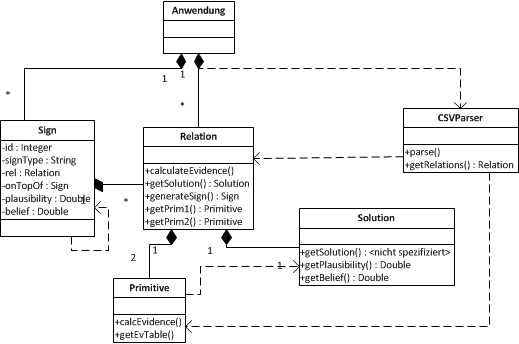
\includegraphics[scale=1]{images/uml.png}
    \caption{UML Diagram der StreetSign Evidence Anwendung}
    \label{sse}
\end{figure}

Ergibt sich daraus ein Schild, wird dieses in einer Liste gespeichert. Nachdem Relationen auf Schilder überprüft wurden, wird geprüft, ob eine Relation zwei Schilder in eine örtliche Relation zu bringen. Für jede \textit{on top} Relation wird geprüft, ob deren erstes und zweites Primitiv ein gültiges Schild enthält. Wenn diese Bedingung erfüllt wird, merkt sich das örtlich obere Schild, dass und welches Schild sich unter ihm befindet.\
\
Am Ende wird über alle Schilder iteriert und ausführlich die bekannten Informationen zu den erkannten Schildern ausgegeben.



	
	
	\clearpage
	\chapter{Appendix}
	{
	% prevents the appendix from displaying footnotemarks
	\let\footnotemark\relax

		% Anhang
		%\clearpage
		\pagenumbering{roman}
	
		% Abbildungsverzeichnis
		\listoffigures
		\addcontentsline{toc}{section}{Abbildungsverzeichnis}
		
		% Quellcodeverzeichnis
	
		\lstlistoflistings
		\addcontentsline{toc}{section}{Quellcodeverzeichnis}
		
		
		% Literaturverzeichnis
		%\clearpage
		%\phantomsection
		%\addcontentsline{toc}{section}{Literaturverzeichnis}
		%\begin{thebibliography}{---}

%Internetquellen:
% Authorship or Source, Year. Title of web document or web page. [type of medium] (date of update if available) Available at: include web site address/URL (Uniform Resource Locator) [Accessed date]. 
% Pictures:
%Dean, R, 2008 Tales from Topographic Oceans. [electronic print] Available at: <http://rogerdean.com/store/product_info.php?cPath=4&products_id=88> [Accessed 18 June 2008]
% Internal:
% Wolf, C. & Burkard, C., 2012. Monitoring-Dashboard: Documentation, s.l.: Internal Source.
\end{thebibliography}


		
		% Abkürzungsverzeichnis
		% vorher in Konsole folgendes aufrufen: 
		%	makeglossaries makeglossaries dokumentation.acn && makeglossaries dokumentation.glo
	    \newpage	
		\printglossary[type=\acronymtype]
		
		% Glossar
		\newpage
		\printglossary[style=altlist,title=Glossar]
	
	}
	
	

\end{document}

